\section{基于DCM的双足(人形)机器人行走轨迹生成}
    该章主要根据文献\cite{englsbergerThreedimensionalBipedalWalking2013}的内容进行重新整理和复现,下面介绍相关内容。
    \subsection{DCM基本动力学方程的推导与几种特征点的定义}
        \subsubsection{DCM(运动发散量)的定义}
            DCM(Divergent Component of Motion),将其定义为相对机器人质心的偏移点,其定义式如下:
            \begin{equation}
                \boldsymbol{\xi }=\boldsymbol{x}+b\boldsymbol{\dot{x}}
                \label{equ2-1}
            \end{equation}

            式\eqref{equ2-1}变形后可得到质心的动力学方程:
            \begin{equation}
                \boldsymbol{\dot{x}}=-\frac{1}{b}\left( \boldsymbol{x}-\boldsymbol{\xi } \right) 
                \label{equ2-2}
            \end{equation}
            其中,当$b>0$时可得到稳定的一阶动力学方程。

            将式\eqref{equ2-1}求一阶导并代入$m\boldsymbol{\ddot{x}}=\boldsymbol{F}$可得DCM动力学方程:
            \begin{equation}
                \boldsymbol{\dot{\xi}}=-\frac{1}{b}\boldsymbol{x}+\frac{1}{b}\boldsymbol{\xi }+\frac{b}{m}\boldsymbol{F} 
                \label{equ2-3}
            \end{equation}
        \subsubsection{eCMP的定义}
            eCMP(Enhanced Centroidal Moment Pivot Point),与式\eqref{equ1-1}中的外力定义形式类似,此处
            将接触作用外力与eCMP定义联系,其关系定义如下,其中$s>0$且为常数:
            \begin{equation}
                \boldsymbol{F}_{ext}=s\left( \boldsymbol{x}-\boldsymbol{r}_{ecmp} \right) 
                \label{equ2-4}
            \end{equation}

            再将上式加上重力所求得合力的代入式\eqref{equ2-3}可得下式\eqref{equ2-5a},再选择
            常数$s=\frac{m}{b^2}$可化简得下式\eqref{equ2-5b}:
            \begin{subequations}
                \begin{align}
                    \boldsymbol{\dot{\xi}} &= \left( \frac{bs}{m}-\frac{1}{b} \right) \boldsymbol{x}+\frac{1}{b}\boldsymbol{\xi }-\frac{bs}{m}\boldsymbol{r}_{ecmp}+b\boldsymbol{g}
                    \label{equ2-5a}\\
                    \boldsymbol{\dot{\xi}} &= \frac{1}{b}\boldsymbol{\xi }-\frac{1}{b}\boldsymbol{r}_{ecmp}+b\boldsymbol{g}
                    \label{equ2-5b}
                \end{align}
            \end{subequations}
        \subsubsection{VRP的定义}
            引入VRP(Virtual Repellent Point)来进一步化简上式\eqref{equ2-5b},定义VRP如下:
            \begin{equation}
                \boldsymbol{r}_{vrp}=\boldsymbol{r}_{ecmp}+\left[ \begin{matrix}
                    0&		0&		b^2g\\
                \end{matrix} \right] ^T=\boldsymbol{r}_{ecmp}+\left[ \begin{matrix}
                    0&		0&		\varDelta z_{vrp}\\
                \end{matrix} \right] ^T
                \label{equ2-6}
            \end{equation}
            将其代入式\eqref{equ2-5b}可得最终形式的DCM动力学方程:
            \begin{equation}
                \boldsymbol{\dot{\xi}}=\frac{1}{b}\left( \boldsymbol{\xi }-\boldsymbol{r}_{vrp} \right) =\sqrt{\frac{g}{\varDelta z_{vrp}}}\left( \boldsymbol{\xi }-\boldsymbol{r}_{vrp} \right)
                \label{equ2-7}
            \end{equation}
            其中$b=\sqrt{\frac{\varDelta z_{vrp}}{g}}$将其代入式\eqref{equ2-4}则可得所有合外力:
            \begin{subequations}
                \begin{align}
                    \boldsymbol{F}&=\frac{m}{b^2}\left( \boldsymbol{x}-\boldsymbol{r}_{vrp} \right) 
                    \label{equ2-8a}\\
                    \boldsymbol{F}&=\frac{mg}{\varDelta z_{vrp}}\left( \boldsymbol{x}-\boldsymbol{r}_{vrp} \right) 
                    \label{equ2-8b}
                \end{align}               
            \end{subequations}
            
            最后的质心CoM动力学方程为:
            \begin{equation}
                \boldsymbol{\dot{x}}=-\sqrt{\frac{g}{\varDelta z_{vrp}}}\left( \boldsymbol{x}-\boldsymbol{\xi } \right) 
                \label{equ2-9}
            \end{equation}

            所有特征点的示意图如下所示:
            \begin{figure}[h] 
                \centering
                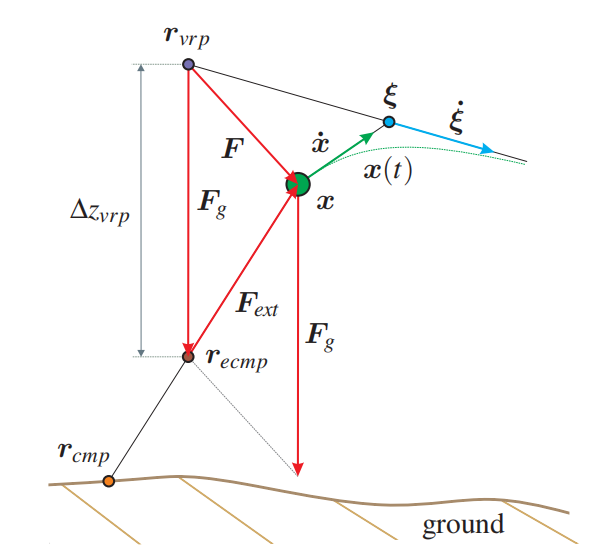
\includegraphics[scale=0.5]{2021-08-17-10-53-23.png}
                \caption{所定义特征点的示意图} \label{fig2-1}
            \end{figure}
    \subsection{几种不同支撑类型下的DCM、CoM轨迹生成}
        \subsubsection{单点支撑SS(Single Support)情形}
            假设机器人的足为单点或支撑点位于脚掌中心,机器人角动量变化为0,且随着双脚切换时支点的移动是
            瞬时的(没有双脚同时受力的情形),则此时令脚支撑点$\boldsymbol{r}_{f,i}$、压力中心$\boldsymbol{r}_{cop}$(Center of Pressure)、
            中心动量支点$\boldsymbol{r}_{cmp}$(Centroidal Moment Pivot Point)以及$\boldsymbol{r}_{ecmp}$重合,这几种点
            的作用示意图如下图\ref{fig2-2a}所示,重合情况见下图\ref{fig2-2b},该方法使得CoP为常量,接触外力总通过质心。
            \begin{figure}[h] 
                \centering
                \subfloat[CoP、CMP、eCMP等点的定义]{
                    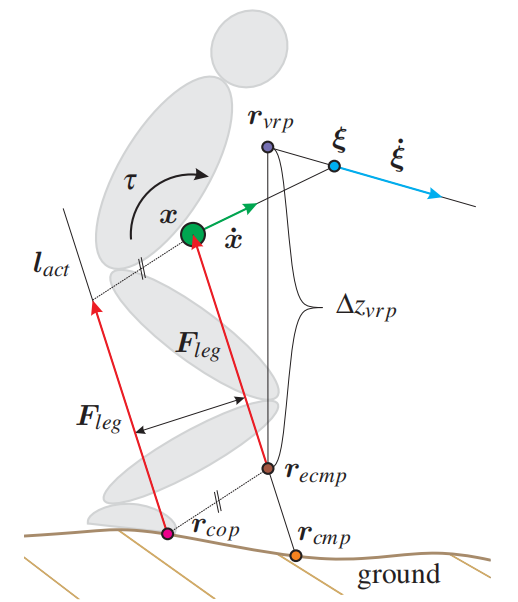
\includegraphics[scale=0.4]{2021-08-17-11-55-16.png}
                    \label{fig2-2a}
                }
                \vspace{10pt} %两图的竖直间隔
                \subfloat[单点支撑时各点重合]{
                    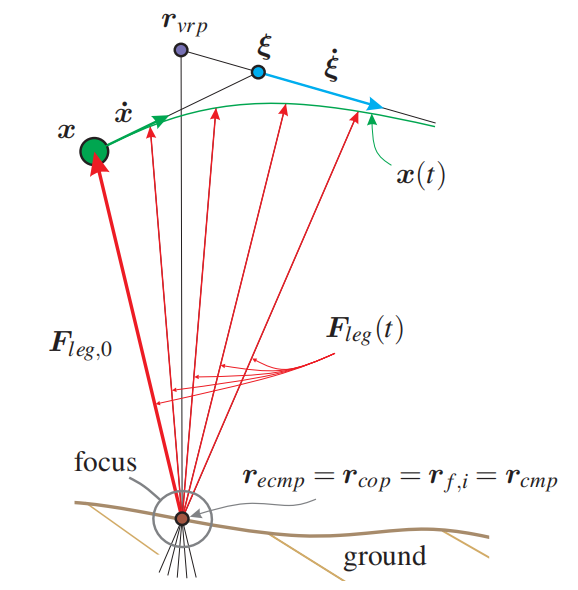
\includegraphics[scale=0.4]{2021-08-17-11-57-17.png}
                    \label{fig2-2b}
                }
                \caption{各点定义及单点支撑的示意图} \label{fig2-2}
            \end{figure}

            首先设定N个落脚点$\boldsymbol{r}_f,i$,限定单点支撑时VRP的位置为该支撑点竖直偏移$\varDelta z_{vrp}$(因为此时CoP与eCMP重合)
            即$z_{vrp,d,i}=z_{f,i}+\varDelta z_{vrp}$,由此VRP的位置在第$i$个支撑点作用时为常量,求解方程\ref{equ2-7}可得:
            \begin{equation}
                \boldsymbol{\xi }\left( t \right) =\boldsymbol{r}_{vrp}+e^{\sqrt{\frac{g}{\varDelta z_{vrp}}}t}\left( \boldsymbol{\xi }\left( 0 \right) -\boldsymbol{r}_{vrp} \right)
                \label{equ2-10}
            \end{equation}
            设定每一段的单个支撑点作用时间为$t_{step,i}$,则上述$t\in \left[ 0,t_{step,i} \right]$。设定最后机器人在第N个支撑点停下,
            下标$d$表示目标值(desired),$eos$表示end of support,此时$\boldsymbol{\xi}_{d,eos,N-1}=\boldsymbol{r}_{vrp,d,N}$,
            可以通过向后迭代推算出每一段支撑运动的DCM起始值$\boldsymbol{\xi}_{d,ini,N-1}$与终止值$\boldsymbol{\xi}_{d,eos,N-1}$,
            根据式\ref{equ2-10}建立迭代式如下:
            \begin{equation}
                \boldsymbol{\xi }_{d,eos,i-1}=\boldsymbol{\xi }_{d,ini,i}=\boldsymbol{r}_{vrp,d,i}+e^{-\sqrt{\frac{g}{\varDelta z_{vrp}}}t_{step,i}}\left( \boldsymbol{\xi }_{d,eos,i}-\boldsymbol{r}_{vrp,d,i} \right) 
                \label{equ2-11}
            \end{equation}
            再将迭代结果代回式\ref{equ2-10}并求导可得到DCM在每段的动力学解,即得到DCM轨迹:
            \begin{subequations}
                \begin{align}
                    \boldsymbol{\xi }_{d,i}\left( t \right) &=\boldsymbol{r}_{vrp,d,i}+e^{\sqrt{\frac{g}{\varDelta z_{vrp}}}\left( t-t_{step,i} \right)}\left( \boldsymbol{\xi }_{d,eos,i}-\boldsymbol{r}_{vrp,d,i} \right) 
                    \label{equ2-12a}\\
                    \boldsymbol{\dot{\xi}}_{d,i}\left( t \right) &=\sqrt{\frac{g}{\varDelta z_{vrp}}}e^{\sqrt{\frac{g}{\varDelta z_{vrp}}}\left( t-t_{step,i} \right)}\left( \boldsymbol{\xi }_{d,eos,i}-\boldsymbol{r}_{vrp,d,i} \right) 
                    \label{equ2-12b}
                \end{align}
            \end{subequations}
            文献\cite{englsbergerThreedimensionalBipedalWalking2013}中的示意图如下图\ref{fig2-3}所示,规定好开始时CoM的位置$\boldsymbol{x}_0$以及
            VRP偏移eCMP的高度$\varDelta z_{vrp}$便可完成规划,可取$\varDelta z_{vrp}$为机器人单(双)腿直立站立静止时CoM与eCMP或支撑点的相对高度,使以上
            模型成立,到终点时CoM速度为零,DCM、CoM与VRP重合(DCM先与VRP重合然后COM跟随一段时间才与DCM重合)。由于初始的DCM位置由脚步点规划后的反向迭代结果确定,因此初始点$\boldsymbol{x}_0$的选择决定了
            初始CoM速度$\boldsymbol{\dot{x}}_0$。
            \begin{figure}[h] 
                \centering
                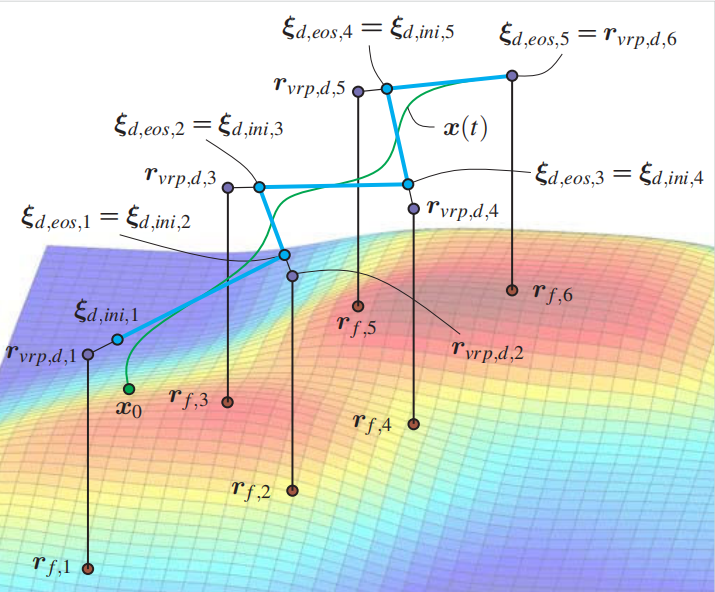
\includegraphics[scale=0.3]{2021-08-17-14-26-05.png}
                \caption{单点支撑DCM轨迹规划示意图} \label{fig2-3}
            \end{figure}

            利用python编写相关程序,预先给定6个落脚点,每段步利用4阶龙格库塔方法求解CoM的轨迹,当DCM到达终点之后一段的CoM轨迹则直接用修改Eular格式
            的单步迭代法求解,具体结果如下图\ref{fig2-4}所示,显示了各个点、每步的时间以及总时间等信息。
            \begin{figure}[h] 
                \centering
                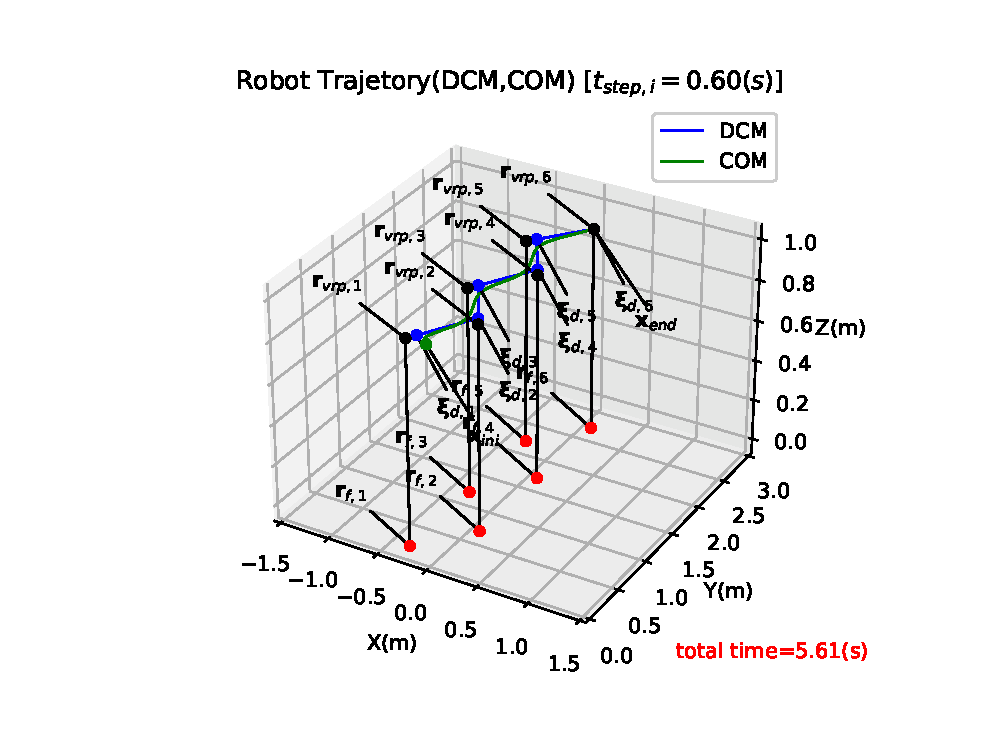
\includegraphics[scale=0.6]{DCM_SS.eps}
                \caption{复现单点支撑DCM轨迹规划图} \label{fig2-4}
            \end{figure}
        \subsubsection{连续双点支撑DS(Double Support)情形}
            

